\documentclass{IEEEtran}
\usepackage[utf8]{inputenc}
\usepackage[pdftex]{hyperref}
\usepackage{algorithmic}
\usepackage{amssymb}
\usepackage{flushend}
\usepackage{graphicx}

\hypersetup{
	colorlinks,
	linkcolor=blue,
	pdfauthor={Davide Pesavento \& Martina Astegno},
	pdftitle={Conductor}
}

\newcommand{\Conductor}{\textsl{Conductor}}
\newcommand{\Probe}{\textsl{Probe}}

\title{\Conductor{}: an automatic audio routing system \\
	based on the RSSI of a passive Bluetooth device}

\author{
	Davide~Pesavento, Martina~Astegno \\
	Università degli Studi di Padova \\
	Corso di Laurea Magistrale in Informatica \\
	\{dpesaven,mastegno\}@studenti.math.unipd.it
}


\begin{document}

\maketitle

\begin{abstract}
In this paper we present a distributed application that shows how the Bluetooth technology can be used to approximately locate a person wearing a Bluetooth device (e.g.\ a smartphone) among a predefined set of rooms. The final result we achieved is the ability to automatically reroute the output of an audio player from one room to another, according to the person's movements over time.
\end{abstract}

%\begin{IEEEkeywords} % normally used for peerreview paper
%Bluetooth, BlueZ, DBus, PulseAudio, audio routing, smartphone.
%\end{IEEEkeywords}
%\IEEEpeerreviewmaketitle


\section{Introduction}

\subsection{Example of a usage scenario}
Jessica is a modern housewife who likes listening to music while doing the housework. Her house is quite big though, and with just one hi-fi in the living room, she cannot hear the music loud enough when she is working in some other rooms. This issue is a major nuisance to her listening experience.

\textbf{\Conductor{}} is exactly what she is looking for: she just needs to install a special kind of speaker in each room and, as long as she keeps her Bluetooth-equipped mobile phone in her pocket, she can freely move from room to room and the music smoothly follows her without interruptions.

\subsection{Short-range device discovery: Bluetooth}
\textbf{Bluetooth} is an open specification for a RF-based system that provides the network infrastructure to enable short range wireless communication of data and voice. It includes a hardware component and a software component. The specification also describes usage models and user profiles for these models.
Bluetooth supports two kinds of links: \textit{Asynchronous Connectionless} (ACL) links for data transmission and \textit{Synchronous Connection Oriented} (SCO) links for audio/voice transmission. Figure~\ref{btstack} shows the various layers of Bluetooth protocol suite.

Bluetooth hardware uses \textit{Frequency Hopping Spread Spectrum} (FHSS) to avoid any interferences. A Bluetooth channel is divided into time slots each 625 microseconds in length. The devices hop through these timeslots making 1600 hops per second. This trades bandwidth efficiency for reliability, integrity and security.

\begin{figure}
\centering
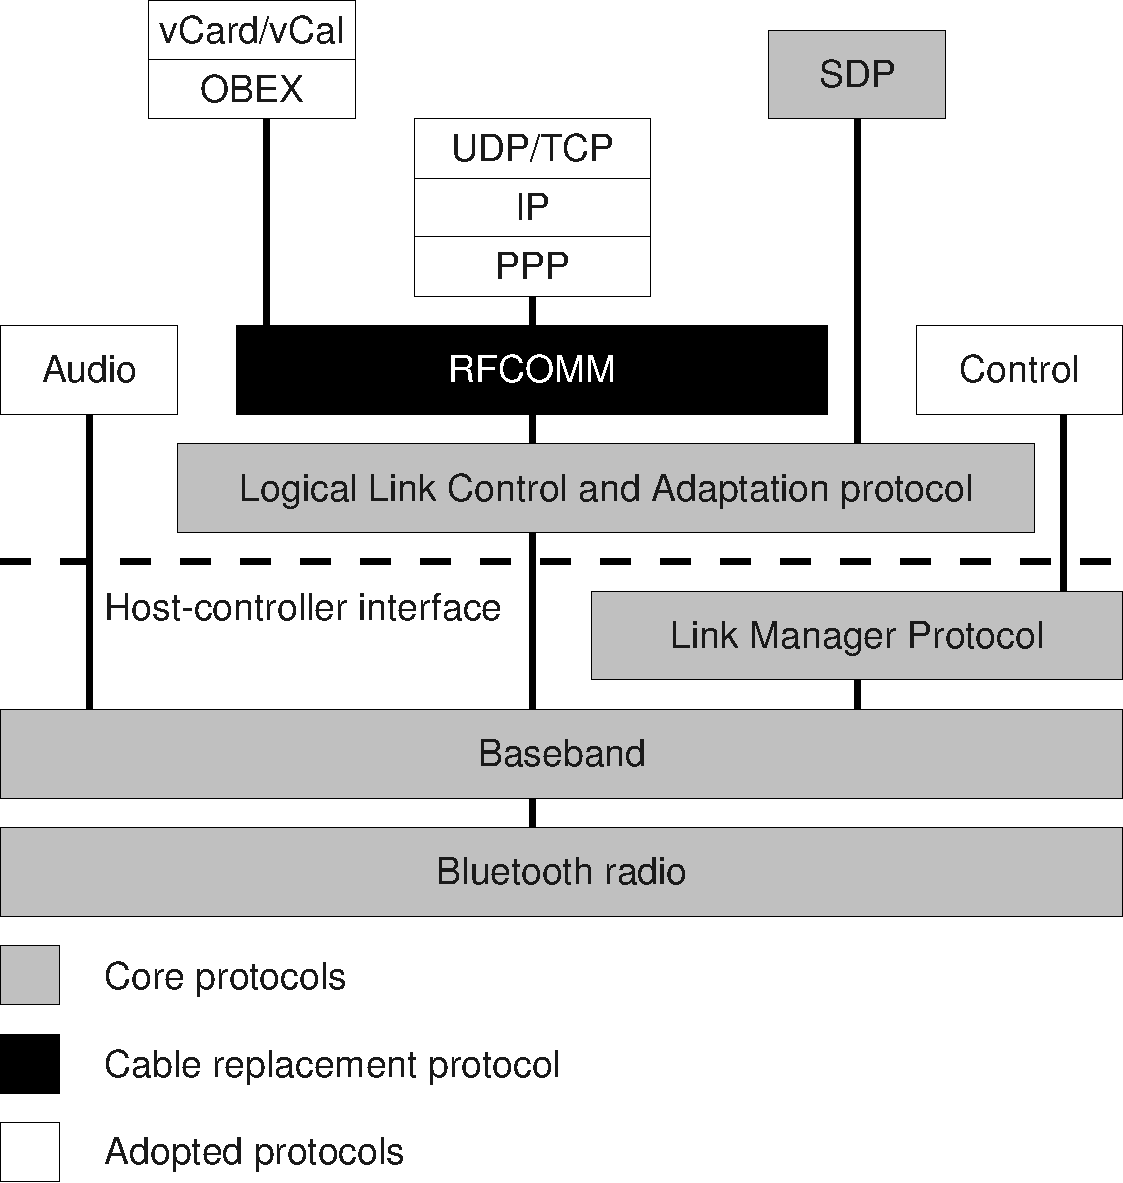
\includegraphics[width=.9\columnwidth]{BTstack}
\caption{Bluetooth protocol stack}
\label{btstack}
\end{figure}

In our project we adopted \textbf{BlueZ} version 4 or later, the official Linux Bluetooth stack implementation, that provides support for the core Bluetooth layers and protocols. It is flexible, modular and efficient. Current versions of BlueZ consist of many separate modules, for example:
\begin{itemize}
\item Bluetooth kernel subsystem core
\item L2CAP and SCO audio kernel layers
\item RFCOMM, BNEP, HIDP kernel implementations
\item HCI UART, USB, PCMCIA and virtual device drivers
\item Bluetooth and SDP userspace daemon (\texttt{bluetoothd})
\item Configuration and testing utilities
\item Protocol decoding and analysis tools
\end{itemize}

\subsection{Audio routing: PulseAudio}
\textbf{PulseAudio} is a cross-platform, networked sound server. A sound server is basically a proxy for sound applications. It allows to do advanced operations on sound data as it passes between an application and the hardware. Tasks like transferring the audio to a different machine, changing the sample format or channel count and mixing several sounds into one are easily achieved using a sound server. PulseAudio is designed for Linux systems, but has been ported to Microsoft Windows, MacOS~X, Solaris, FreeBSD and other POSIX-compliant platforms. Figure~\ref{pa} depicts a high level overview of PulseAudio architecture.

\begin{figure}
\centering
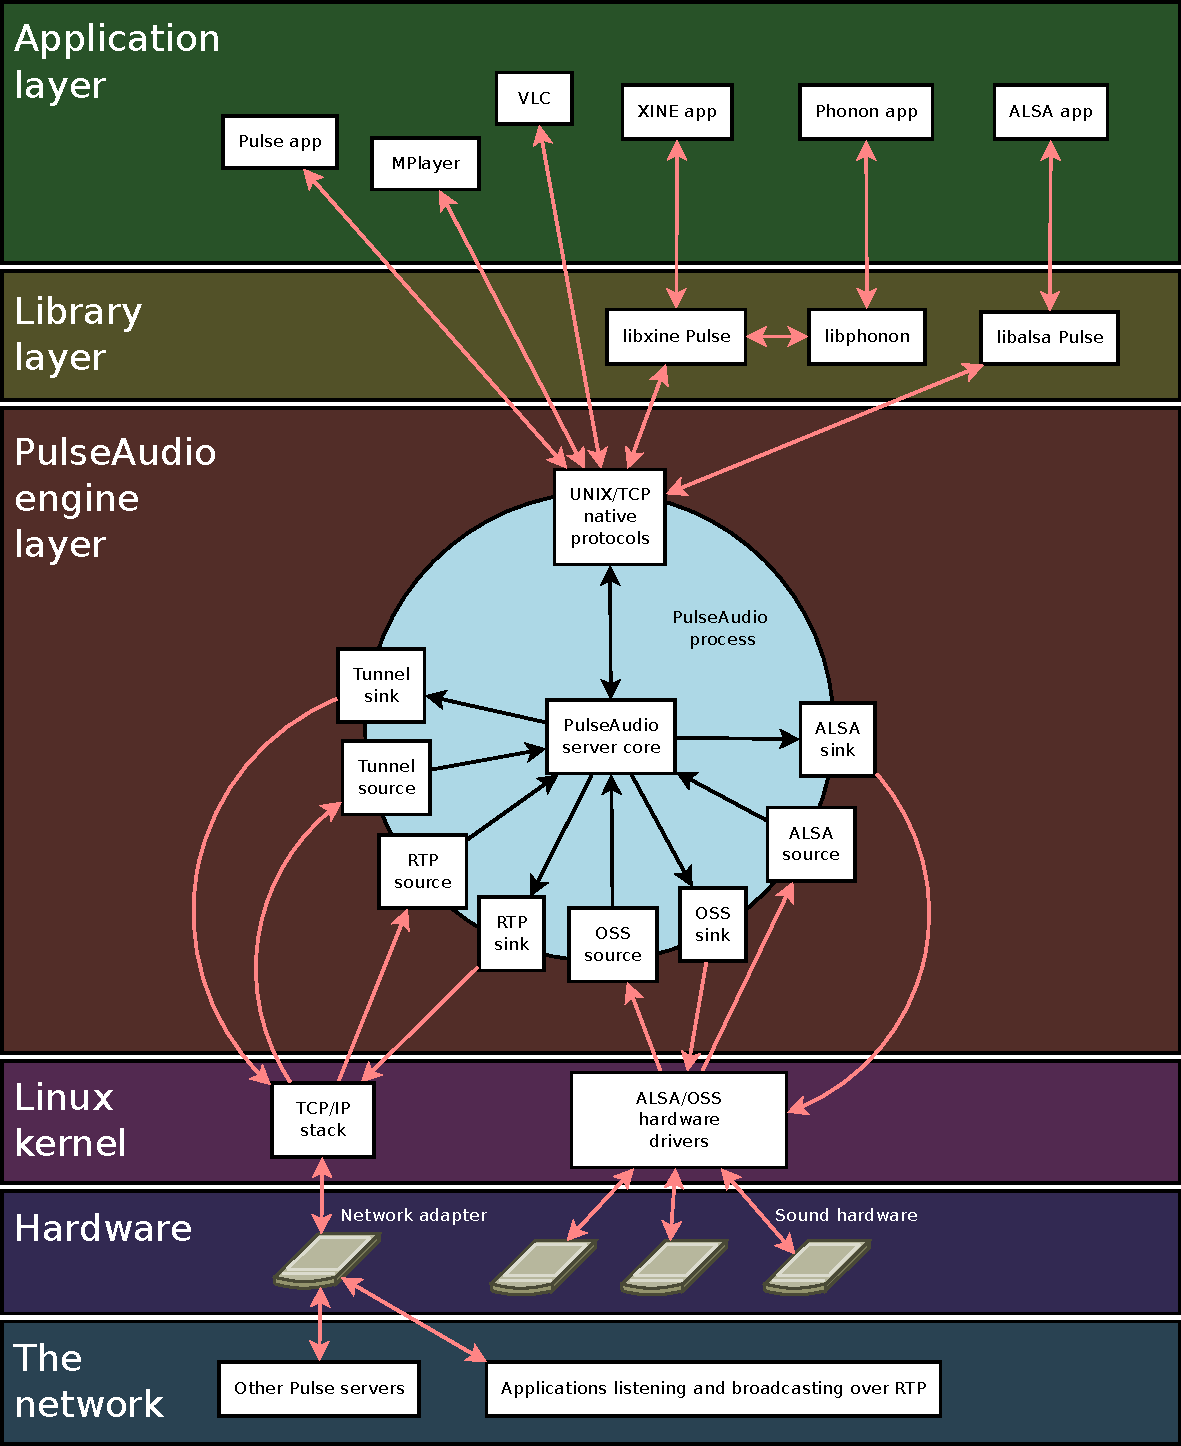
\includegraphics[width=\columnwidth]{PulseAudio}
\caption{High-level PulseAudio architecture}
\label{pa}
\end{figure}


\section{General architecture}
In this chapter we will explain the high-level architecture of our prototype and the major design choices we have made during its development.

The prototype can be divided into 3 primary components, which will be described in greater detail in the next sections, plus a \textsl{Qt4} graphical user interface, that will be left out because it does not contain any noteworthy functionalities.

\begin{figure*}
\centering
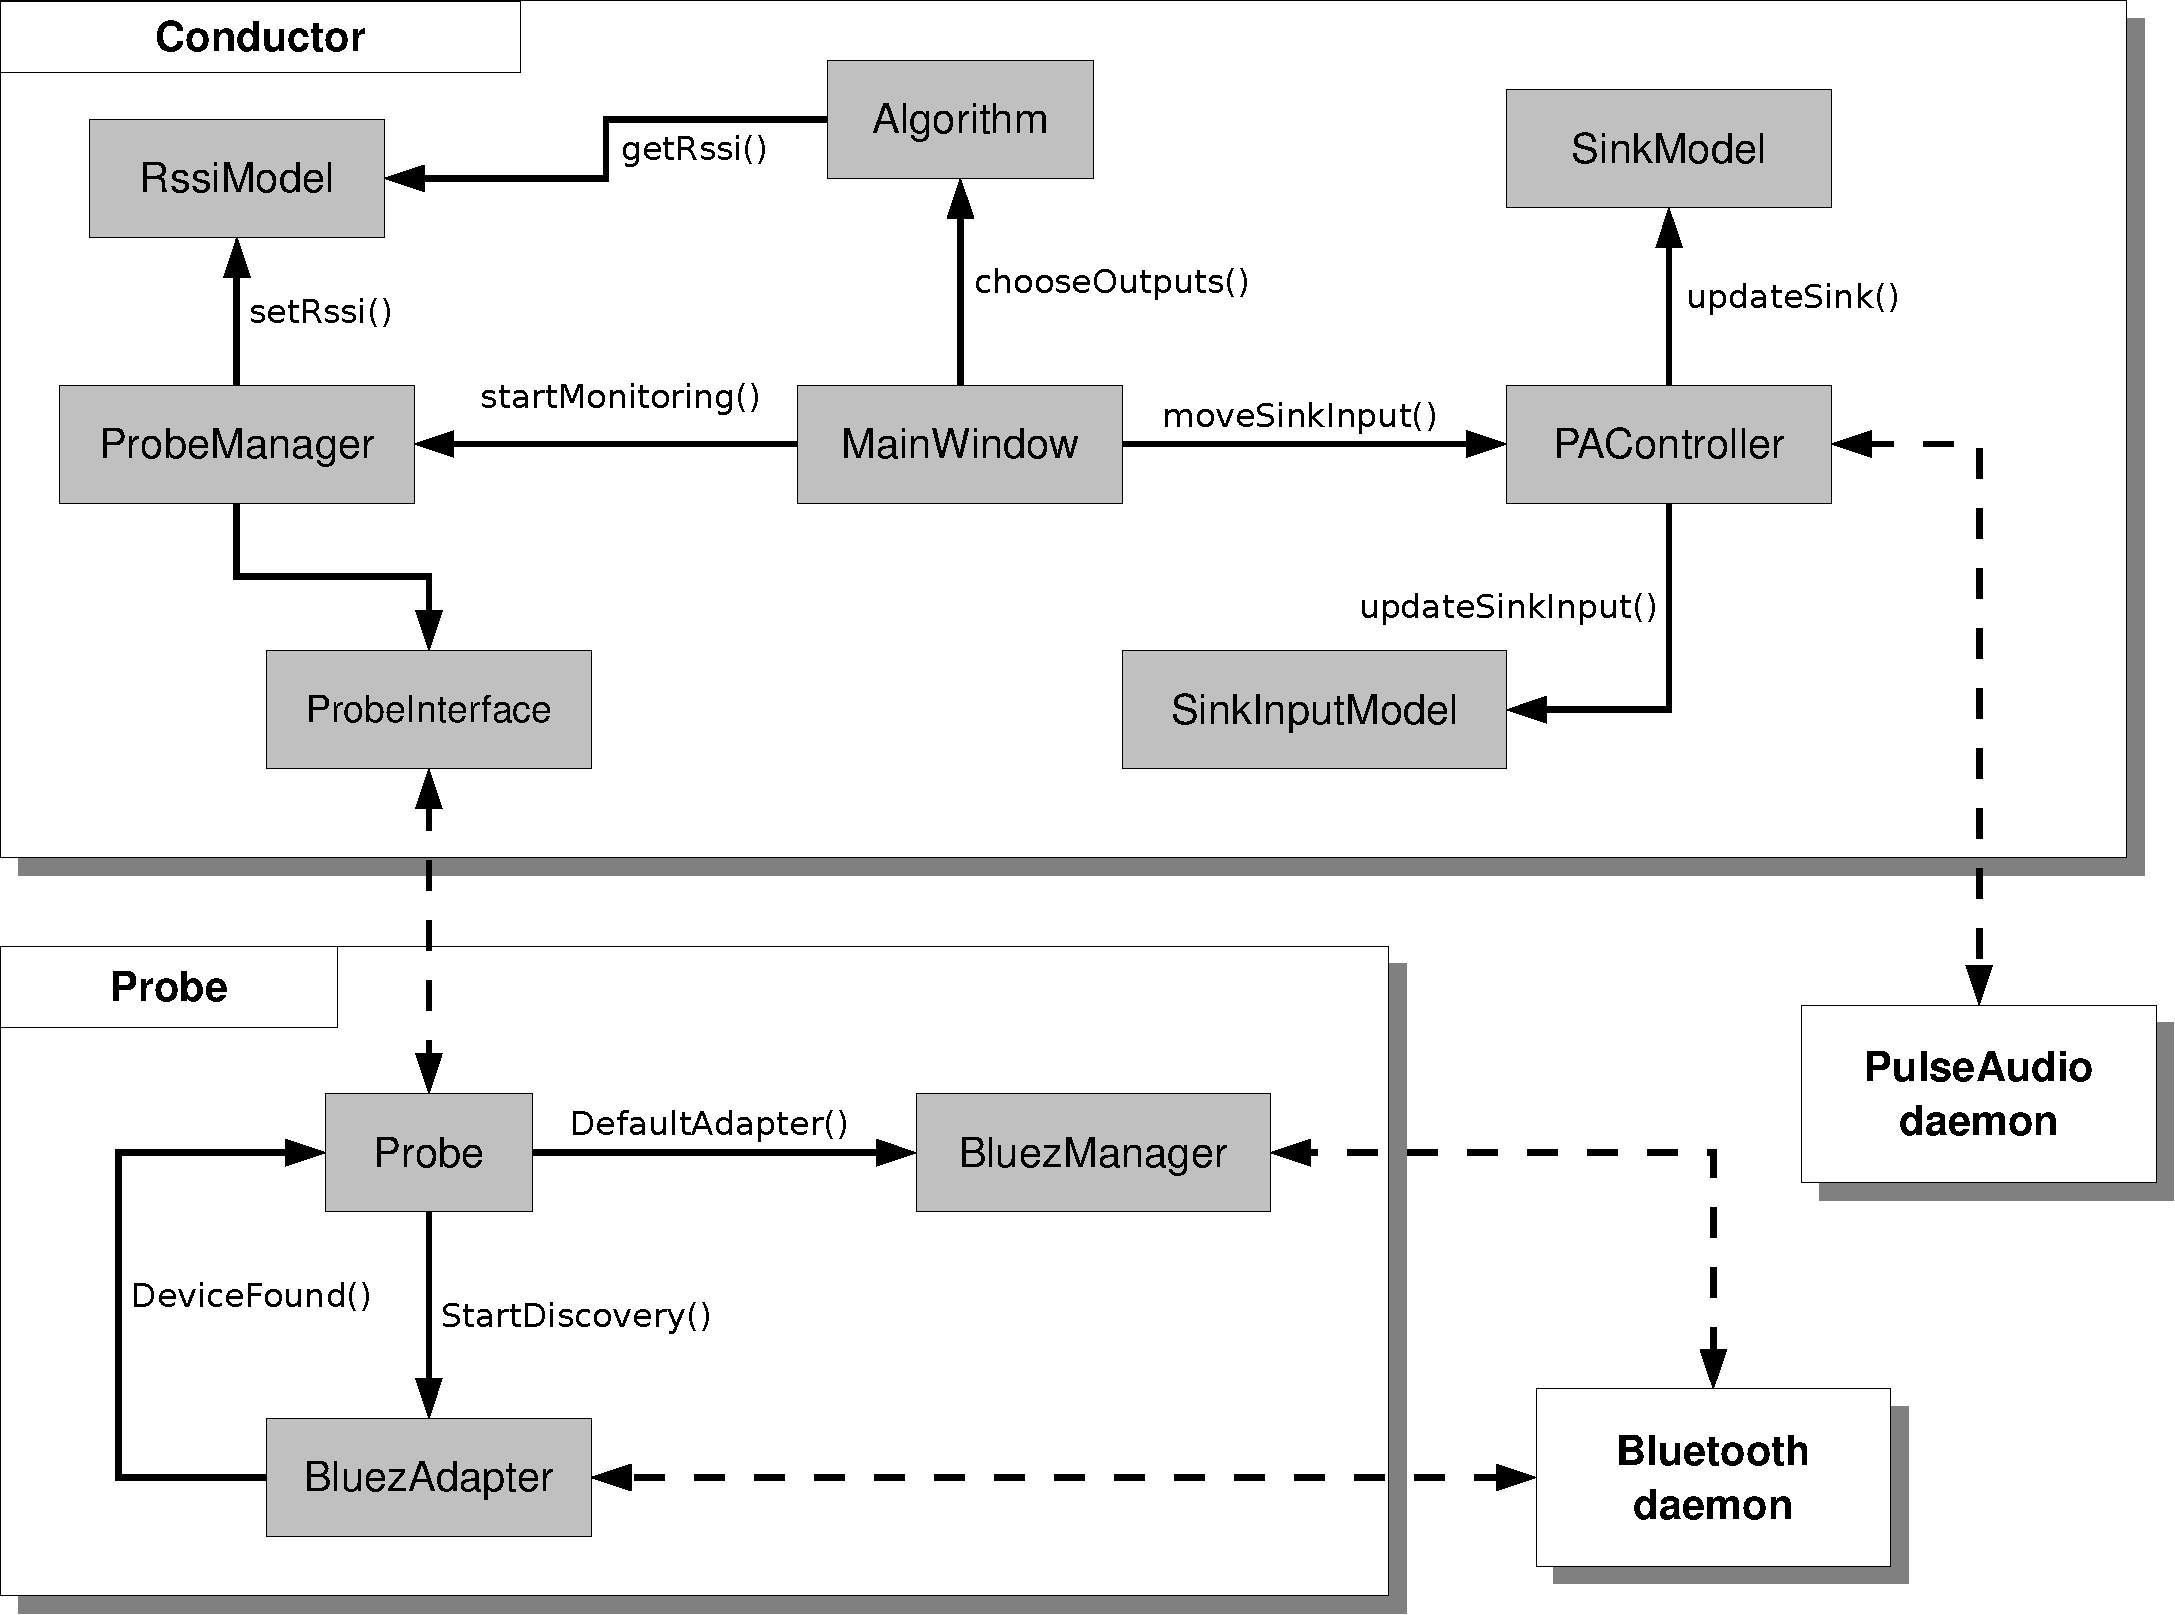
\includegraphics[width=.85\textwidth]{Arch}
\caption{Main classes and interactions between them}
\label{arch}
\end{figure*}

\subsection{Bluetooth module}
\label{btmod}
The Bluetooth component deals with the discovery of monitored devices. In particular, the class \texttt{ProbeManager} connects to all available Bluetooth adapters upon startup and then sends them appropriate commands to setup or teardown a discovery session.

Since most of these adapters are not directly visible to \Conductor{} but they are instead wired up to different machine that is in turn connected to the main application via TCP, the prototype relies on another application, named \textbf{\Probe{}}, which is basically a proxy between \Conductor{} and the Bluetooth adapters. An instance of \Probe{} must be running on each node of the network that has an adapter attached to it. On the whole the application is tiny, efficient and has no GUI, thus it should even be possible to run it on embedded devices.

\texttt{ProbeManager} interacts with each \Probe{} through an object of type \texttt{ProbeInterface}, derived from \texttt{QxtRPCPeer}, that completely hides the details of the network protocol used to communicate with the remote side, thus greatly simplifying the implementation.

\Probe{} uses \textbf{DBus} to interface with BlueZ. When asked to, it begins monitoring the discoverable devices by calling \texttt{BluezAdapter::StartDiscovery()} and then waits to be notified about their presence by the signal \texttt{DeviceFound}. While a discovery session is active, the BlueZ daemon also notifies the requesting client each time the detected RSSI (\textit{Received Signal Strength Indicator}) changes: this allows sending the updated value to the main application as quickly as possible.

\subsection{PulseAudio module}
\label{pamod}
The PulseAudio component has three main responsibilities:
\begin{itemize}
	\item \textbf{querying} the daemon for the list of available sinks and audio streams and keeping such information up-to-date;
	\item \textbf{loading} PulseAudio modules with the appropriate configuration and \textbf{unloading} them when they are no longer needed;
	\item \textbf{redirecting} an audio stream from one sink to another when requested by the application's logic.
\end{itemize}
All these operations are performed asynchronously. To keep track of in-flight operations, PulseAudio libraries return a reference-counted \texttt{pa\_operation} object for each of them.

Although the full introspection API is very powerful, it is also rather complex to use, being written in plain C and heavily relying on callbacks to implement asynchronous notifications. Therefore we developed a thin C++ layer on top of it, to simplify its usage by the rest of the application.

The two basic data structures at the bottom of PulseAudio, \texttt{pa\_sink} and \texttt{pa\_sink\_input}, are wrapped respectively by the classes \texttt{Sink} and \texttt{SinkInput}.

Asynchronous operations are wrapped in a similar way: each kind of operation is encapsulated by a different class, which hides all the details about how to submit that operation to the daemon and how to handle the result or a possible error. These classes are then organized into a simple hierarchy, with a common abstract base class (\texttt{PAOperation}) that exposes a unified interface to execute operations, without having to worry about their type. The two most interesting \texttt{PAOperation} subclasses are:
\begin{itemize}
	\item \texttt{LoadModuleOperation}: loads a PulseAudio module to accomplish a specific task. In particular, our application uses the two following modules:
	\begin{itemize}
		\item \texttt{module-tunnel-sink} creates a new sink that forwards its input to the other end of the tunnel via a TCP connection; it requires a running PulseAudio daemon on the remote side.
		\item \texttt{module-combine} allows playing the same audio stream through two or more sinks simultaneously. A new virtual sink is allocated and all data written to it is forwarded to every connected sink.
	\end{itemize}
	\item \texttt{MoveOperation}: redirects a \texttt{SinkInput} from the current sink to the specified one.
\end{itemize}

On top of everything, class \texttt{PAController} is the façade for the whole module and provides a further level of abstraction. Internally it uses the classes described above, thus avoiding most of the complexity of interfacing with PulseAudio libraries directly. Its API is simple to use and consists mainly of these two methods:
\begin{itemize}
\item[$\vartriangleright$] \texttt{createTunnel(QByteArray server)}
\item[$\vartriangleright$] \texttt{moveSinkInput(SinkInput input, QList<QByteArray> speakers)}
\end{itemize}
The first method executes a \texttt{LoadModuleOperation} to create a tunnel sink towards the specified server. The second method redirects an arbitrary \texttt{SinkInput} to all the sinks corresponding to the specified list of speakers; this is accomplished using a \texttt{MoveOperation}, possibly preceded by the loading of an instance of \texttt{module-combine} if the list contains two or more speakers.

In order to implement these features, \texttt{PAController} has often the need to perform not just a single atomic operation but many of them. However these operations must usually be executed in a well-defined sequential order. This is quite difficult to achieve directly, due to the asynchronous nature of PulseAudio APIs. Therefore we designed a dedicated class (\texttt{PAOperationQueue}) which, while keeping an asynchronous design, is able to safely handle a queue of operations by submitting them only when all their dependencies have been satisfied, i.e.\ after the daemon notifies that all the operations on which they depend have been completed.

\subsection{Output selection algorithm}
\label{algo}
This algorithm is the core of \Conductor{}: it tries to figure out in which room the monitored device is currently located and it selects the speakers that have to start reproducing sound accordingly.

The algorithm runs periodically at configurable intervals and, on each execution, it proceeds as follows. First of all, it obtains the latest RSSI value associated with each room using the method \texttt{RssiModel::getRssi()}. Then the values are sorted and a heuristics is applied to the highest ones. This heuristics takes into consideration the relative position of rooms, discarding any invalid combinations from the set of selected outputs (e.g.\ it does not make any sense to reproduce simultaneously in two rooms which are not contiguous). Finally, if the resulting set of rooms is different from the current one, the \texttt{outputsChanged} signal is emitted, eventually causing the invocation of \texttt{PAController::moveSinkInput()}.

The following pseudo-code shows more precisely how the implemented algorithm works.
\vspace{3mm}

\textit{Short description of all variables involved in the algorithm}
\begin{itemize}
\item \texttt{adjacencyMap}: maps each room to the list of its adjoining rooms.
\item \texttt{best}: a set containing the rooms that have the first \texttt{maxSimultaneousSpeakers} highest RSSI values.
\item \texttt{curRooms}: the rooms where the audio stream is currently being played.
\item \texttt{maxRetries}: maximum number of retries (see description of \texttt{retryCount}); when exceeded the playback should be stopped.
\item \texttt{maxSimultaneousSpeakers}: maximum number of speakers that can be activated simultaneously.
\item \texttt{neighbors}: the set of rooms that are contiguous to at least one room in \texttt{curRooms}.
\item \texttt{outputs}: the new set of rooms chosen by the algorithm to reproduce the stream.
\item \texttt{retryCount}: an integer counter used to delay playback interruption when the device temporarily falls out of range.
\item \texttt{rssiMap}: maps each room to the last RSSI value received by the \Probe{} located inside that room.
\end{itemize}

\vspace{3mm}

\textbf{\textit{Algorithm::chooseOutputs()}}
\begin{algorithmic}[1]
\STATE $retryCount \gets 0$
\STATE $outputs \gets \varnothing$
\STATE $best \gets \varnothing$

\STATE $sorted \gets sort(rssiMap)$
\FOR{$i = 1$ \textbf{to} $maxSimultaneousSpeakers$}
	\STATE $best \gets best \cup sorted[i]$
\ENDFOR

\IF{$best = \varnothing$ \textbf{and} $retryCount < maxRetries$}
	\STATE $retryCount \gets retryCount + 1$
	\STATE $sleep(updateInterval)$
	\STATE \textbf{goto} 4
\ENDIF

\STATE $neighbors \gets \varnothing$
\FORALL{$r \in curRooms$}
	\STATE $neighbors \gets neighbors \cup adjacencyMap[r]$
\ENDFOR

\STATE $outputs \gets best \cap neighbors$
\RETURN $outputs$
\end{algorithmic}


\section{Prototype testing}
Before evaluating the results of the tests performed on the prototype, we will briefly outline the setup needed to run the applications.

\subsection{Hardware requirements}
\label{hwreqs}
During the project specification and development we assumed the availability of a precise hardware setup.

The prototype basically requires:
\begin{itemize}
	\item a Bluetooth \textbf{device} (e.g.\ smartphone), used to determine the room in which the person is currently located. For simplicity, we have considered only one such device, but the prototype can trivially be extended to support an arbitrary number of devices.
	\item a \textbf{central server}, where the audio player and the main \Conductor{} application run.
\end{itemize}
Furthermore, inside each room there must be:
\begin{itemize}
	\item one Bluetooth \textbf{adapter}, used to monitor the RSSI of the device. It must support \textit{HCI inquiries with RSSI reporting}, as documented in the Bluetooth HCI specification.
	\item one \textbf{speaker}, that starts reproducing the audio stream when its room is chosen for playback.
\end{itemize}

\subsection{Software configuration}
The user is required to setup some parameters before starting the main application. Currently, we have not implemented any sophisticated configuration methods, in order to keep the prototype simple, but configuration management is entirely encapsulated inside the class \texttt{Config}, which makes it trivial to implement an alternative and more flexible backend. For the time being, the values can be directly modified inside \texttt{config.cpp} and \texttt{config.h}.

Available configuration keys are:
\begin{itemize}
\item \texttt{maxRetries}: this is directly used in the output selection algorithm to set an upper bound for \texttt{retryCount} (see section~\ref{algo}).
\item \texttt{maxSimultaneousSpeakers}: maximum number of speakers that can be activated simultaneously.
\item \texttt{probesAddresses}: maps each room to the IP address of the \Probe{} instance that is running there.
\item \texttt{roomsNames}: list of names of all rooms; this value is automatically obtained from \texttt{probesAddresses} and rarely needs to be modified.
\item \texttt{roomsTopology}: for each room, it gives the set of rooms that are contiguous to it.
\item \texttt{updateInterval}: the amount of time (in milliseconds) between two consecutive executions of the algorithm.
\end{itemize}

\subsection{Testing procedure}
Due to the lack of appropriate Bluetooth hardware, we were not able to test the prototype as a whole. Nevertheless we did perform some functional tests of the Bluetooth and PulseAudio components separately in a simulated environment.

The testbed consisted of two notebooks equipped with a sound card and a speaker, connected via an Ethernet cable. Each machine represented a different room.

When started in testing mode, the interface of \Conductor{} allows to manually set the RSSI values associated with each room. By changing these values, the user can simulate the movements of the monitored device across rooms and check whether the system reacts correctly. Normally the stream should only be reproduced on the machine with a non-empty RSSI. If neither are empty, it should instead be reproduced on both machines simultaneously.

\subsection{Experimental results}
Overall the prototype proved to be very stable and efficient during every operation. However we discovered two noteworthy issues, probably to be attributed to the technologies we rely upon and not to our implementation.

The first problem is an inherent characteristic of the inquiry method we employed for device monitoring. The RSSI values reported by one adapter for the same device showed a high variance, which makes it difficult to integrate sophisticated heuristics in the algorithm. This could be a major roadblock for applications that need to determine the precise location of the device, but in our case it was not a serious shortcoming, since we just needed an approximation in order to infer the current room.

The second issue involves the redirection of audio streams. Soon we discovered that PulseAudio's \texttt{module-combine} and \texttt{module-tunnel-sink} are not mature enough to ensure a flawless listening experience. Indeed sometimes we heard noticeable latencies and even incorrect resampling when an audio stream had just been moved from one sink to another (possibly virtual) one.


\section{Future work}
In this chapter we will examine some possible future extensions of the project.

\subsection{Real-world testing}
The prototype has been tested through an additional user interface that allows to simulate a person's movements. This interface exposes a monitor with an editable input box for each room. By interacting with it, the user is able to insert an arbitrary RSSI value to simulate his movements among the rooms (the higher the value, the closer he is to the corresponding room). However this is just a simulation, thus the overall system behavior might be slightly different in the real-world case.

In order to improve the consistency and the reliability of test results, it is therefore advisable to perform a more thorough testing session in a real-world scenario. We could not do that due to the lack of a sufficient number of Bluetooth adapters satisfying the hardware requirements outlined in section~\ref{hwreqs}.

A more realistic testing phase could also have highlighted some shortcomings of the current algorithm and would have enabled us to fine-tune it to meet the initial expectations for the project.

\subsection{Multiple monitored devices}
In section~\ref{hwreqs} we assumed that there is only one device to monitor. However we believe that extending the system to be able to locate multiple devices would be a major feature. This entails the necessity of evaluating how different devices could interact, and will eventually require the development of a policy to handle conflicts between them. Once a solution to this potential issue has been found, modifying the current implementation should be trivial because the prototype has already been designed with this extension in mind, so the code is already quite generic and makes very few assumptions about the number of monitored devices.

\subsection{Lightweight control application on device}
Currently the device is only used to locate the person wearing it. It would be interesting to develop a mobile application to give the user a certain degree of control on audio streams. For instance, with this new feature, he should be able to adjust the volume and pause or stop the playback. A further improvement could be constituted by an interface to navigate through the playlist, i.e.\ choosing a specific song or skipping to the next/previous track.


\vspace{5mm}
\section{Conclusions}
The Bluetooth technology has traditionally been considered only as a cable replacement to enable short-range data and voice communications. Our project showed how it can instead be used to detect the position of a person in a contained environment with reasonable approximation. Furthermore, the inquiry method we used resulted in an extremely low power consumption for the monitored device.

PulseAudio proved to be a very advanced sound server, although some of its features were not mature enough to be able to always provide a reliable and glitch-free rerouting of audio streams. In our opinion this is an area of PulseAudio that needs more work.

Overall we believe that our prototype represents a good starting point for future extensions and improvements.


\begin{thebibliography}{1}
\bibitem{BlueZ}
	\emph{BlueZ: the official Linux Bluetooth protocol stack} \\
	\url{http://www.bluez.org/}
\bibitem{BlueZ-DBus}
	Marcel~Holtmann,
	\emph{Playing BlueZ on the D-Bus} \\
	\url{www.kernel.org/doc/ols/2006/ols2006v1-pages-421-426.pdf}
\bibitem{DBusSpec}
	H.~Pennington, A.~Carlsson, A.~Larsson,
	\emph{D-Bus Specification} \\
	\url{http://dbus.freedesktop.org/doc/dbus-specification.html}
\bibitem{PulseAudio}
	\emph{PulseAudio sound server} \\
	\url{http://www.pulseaudio.org/}
\bibitem{PulseAudioModules}
	\emph{PulseAudio modules} \\
	\url{http://pulseaudio.org/wiki/Modules}
\bibitem{PulseAudioDoc}
	\emph{PulseAudio API documentation} \\
	\url{http://0pointer.de/lennart/projects/pulseaudio/doxygen/}
\bibitem{PulseAudioDiagram}
	\emph{How PulseAudio works} (adapted) \\
	\url{http://rudd-o.com/en/linux-and-free-software/how-pulseaudio-works}
\end{thebibliography}

\end{document}
